\chapter{Design Model: Distributed Managed Systems (DREMS)}
\label{chapter:DREMS}

\section{DREMS Component Model}

Timing analysis of component-based software, as presented in this dissertation, is facilitated by the DREMS component model (\iapfull) \cite{DREMS13Software} \cite{ISIS_F6_ISORC:13}. DREMS was designed and implemented for the class of distributed real-time embedded systems that are remotely deployed and characterized by strict timing requirements e.g. a cluster of satellites, UAV swarms, disaster relief robots etc. DREMS is a software infrastructure for the design, implementation, deployment and management of component-based distributed real-time embedded systems. The infrastructure includes design-time modeling tools \cite{ISIS_F6_SFFMT:13} that integrate with a well-defined and fully implemented component model \cite{ISIS_F6_ISORC:13, kumar2014colored} used to build component-based applications. Rapid prototyping and code generation features coupled with a modular runtime platform automate the tedious aspects of the software development and enable robust deployment and operation of mixed-criticality distributed applications. This chapter elaborates on the DREMS component model, the operation execution semantics, and the process scheduling aspects i.e. properties of the DREMS software stack that are relevant for generating a timing analysis model.

%The DREMS component model is based on the Component Integrated ACE ORB (CIAO) \cite{RT_CIAO:04, CIAO_Chap:04} project. CIAO is an implementation of the OMG's Lightweight CORBA Component Model (CCM) \cite{CCM-light:03}. CIAO uses the TAO~\cite{TAO:02} CORBA object request broker (ORB) as its default underlying communication middleware.  With the recent standardization of connector mechanisms~\cite{dds4ccm:09}, CIAO is also able to support asynchronous messaging and the OMG Data Distribution Service (DDS) through its ports. Unlike CIAO, the DREMS component model is not tightly coupled with the CORBA transport mechanisms. All component communication is via ports and connectors \cite{Connectors} enabling a variety of interaction schemes. 

\begin{figure}[h]
	\centering
	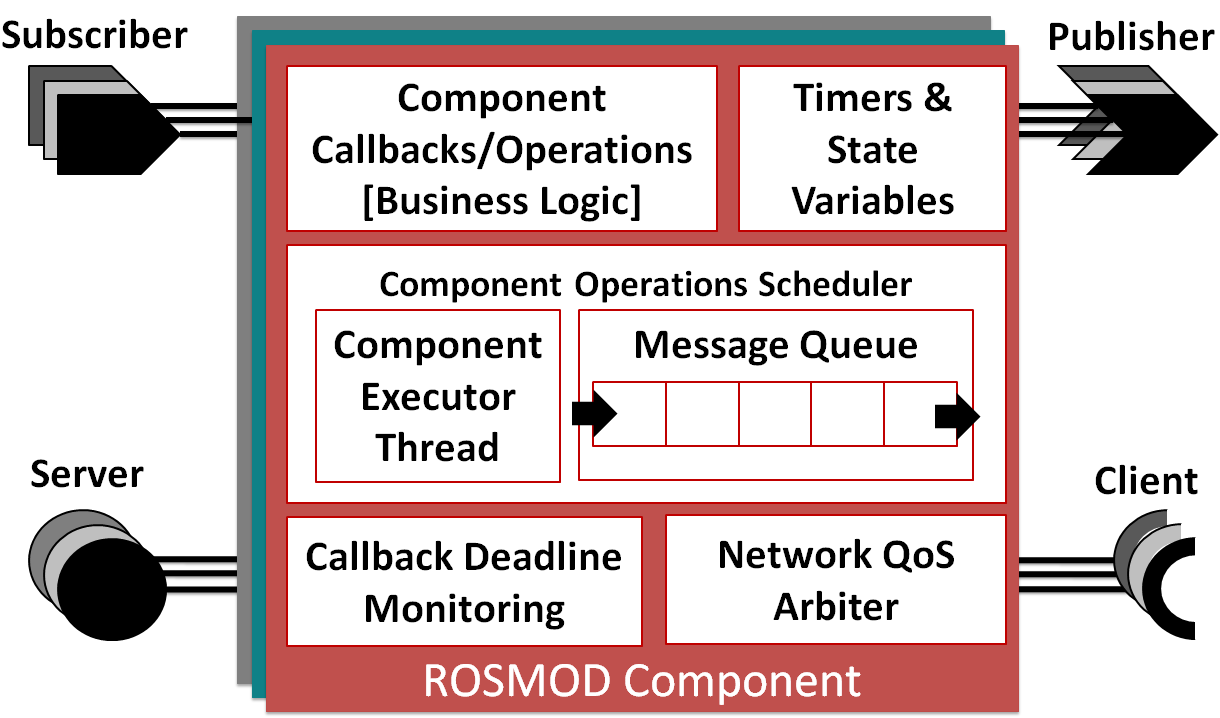
\includegraphics[width=\textwidth]{ROSMOD_Component}
	\caption{DREMS Component}
	\label{fig:DREMS_Component}
\end{figure}


Figure \ref{fig:DREMS_Component} presents a typical DREMS-style component. Component-based software engineering relies on the principle of assembly -- large and complicated systems can be iteratively constructed by composing small reusable component building blocks. Each \emph{component} contains a set of communication ports and interfaces, a message queue, time-triggered event handling and state variables. Using ports, components communicate with the external world. Using interfaces and message passing schemes, components process requests from other components. This interaction mechanism lies at the heart of component-based software. Each DREMS component supports four basic types of ports for interaction with other collaborating components: Facets, Receptacles, Publishers and Subscribers. A component's {\bf facet} is a unique interface that it exposes to its clients. This interface can be invoked either synchronously via remote method invocation (RMI) or asynchronously via asynchronous method invocation (AMI) \cite{waldo1998remote, raje1997asynchronous}. A component's {\bf receptacle} specifies an interface required by the component in order to function correctly. Using its receptacle, a component can invoke operations on other components using either RMI or AMI. A {\bf publisher} port is a single point of data emission. This port emits data produced by a component operation. A {\bf subscriber} port is a single point of data consumption, feeding received data to the associated component. Publishers and Subscribers enable the OMG DDS anonymous publish/subscribe \cite{eugster2003many} style of messaging. More details on this component model can be found in ~\cite{ISIS_F6_ISORC:13}.

\section{Component Execution Semantics}

An \emph{operation} is an abstraction for the different tasks undertaken by a component. These tasks are implemented by the component's source code written by the developer. Application developers provide the functional, \emph{business-logic} code that implements operations on local state variables and inputs received on component ports. For example, a PID controller \cite{aastrom2006advanced} could receive the measured value of a process variable from a \emph{sensor} component, and using the relevant gains and set points (desired value for the process variable), calculate a new state to which an \emph{actuator} component should progress the system. 

In order to service interactions with the underlying framework and with other components, each component has a \emph{message queue}. This queue holds operation requests received from another component i.e. messages, service requests or responses, and timer activations. Each request is characterized by a priority and a deadline. Priority refers to the relative importance of one operation over another within the scope of the component. Deadline refers to the worst-case duration from the arrival of a triggering event to the completion of the response operation. If the execution of the operation takes beyond its deadline to complete, then a \emph{deadline violation} is said to have occurred. 

Each DREMS component has a separate execution thread that handles the execution of all component operations. This executor thread picks the next available request from the message queue and executes the operation to completion i.e. the operation scheduling is non-preemptive. So, all operations in the queue, regardless of priority, need to wait for the currently executing operation to complete. Allowing only a single executor thread per component and enforcing a single-threaded non-preemptive scheduling scheme on the operations helps avoid synchronization primitives for internal state variables and establishes a more easily analyzable system. It is true that multi-threaded solutions to operation scheduling would avoid starvation i.e. operations in the queue will not have to wait forever if the currently executing operation is blocked on a resource. We address such cases in our experimental evaluation (Section \ref{sec:long_running_operations}). However, the DREMS execution semantics is still the more predictable design as it is more easily analyzable. The non-determinism in multi-threaded executions causes a tree of possible behaviors, leading to a common analysis challenge called state space explosion \cite{lin1987protocol}. Keeping the operation execution to a single thread per component bounds the overall number of threads in the system leading to a more tractable analysis. 

\begin{figure}[ht]
	\centering
	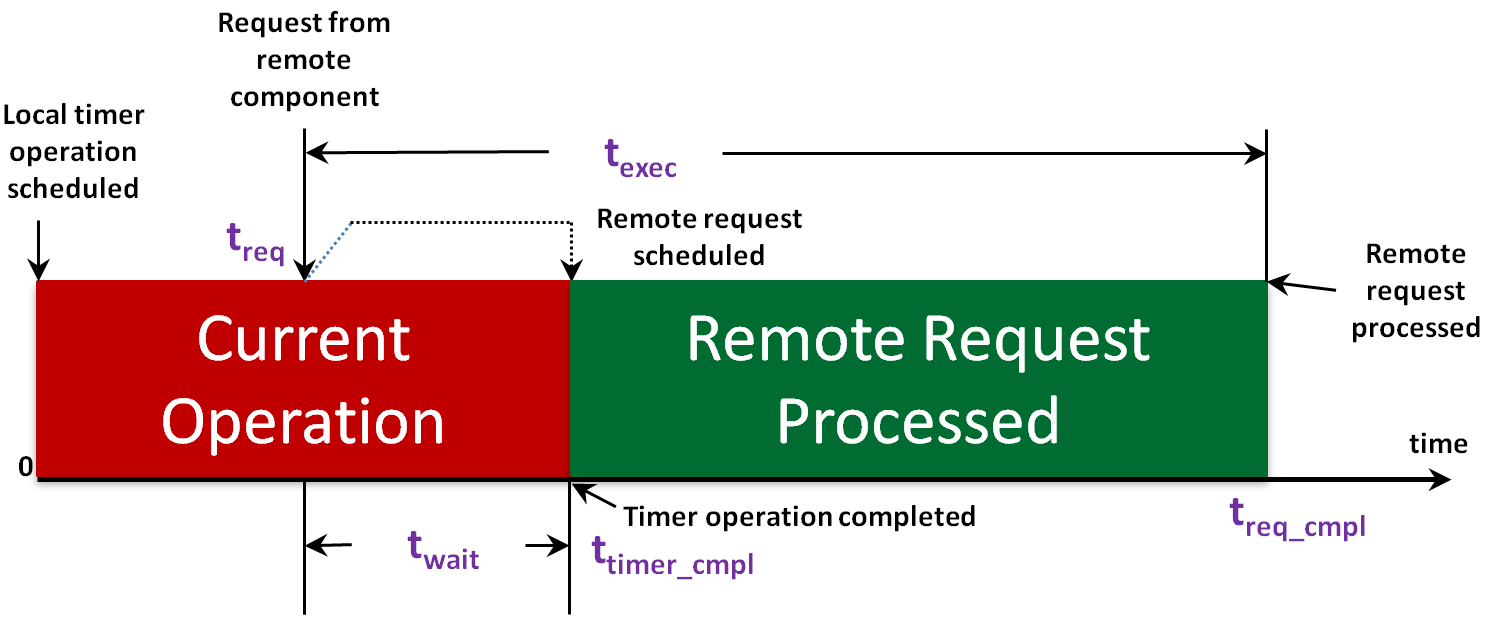
\includegraphics[width=\textwidth]{cop_execution_semantics}
	\caption{Component Operation Execution Semantics: This figure shows the DREMS operation scheduling on an incoming operation request. At some time $t_{i}$, the component executor thread is busy executing an operation -- component operations can be triggered into execution by the (1) expiry of a timer, (2) the arrival of a subscription message, or (3) the arrival of a service request. $t\_{req}$ represents the arrival time of a remote request. $t\_{wait}$ is the wait time of this request in the message queue while the current operation is still executing. $t\_{req\_schld}$ is the time stamp at which the current operation completes executing. At this time, the remote request is finally scheduled for execution. $t\_{req\_cmpl}$ is the time stamp at which the remote request completes. The overall time taken by the component to respond to this request is calculated as: $t\_{wait} + t\_{exec} = t\_{req\_cmpl} - t\_{req}$.}
	\label{fig:cop_execution_semantics}
\end{figure}

Figure \ref{fig:cop_execution_semantics} shows the execution semantics of a component operation executed on the component's executor thread. Simplifying assumptions include that this component is the only component thread executing on the CPU, assuming a single core CPU. This is a simple scenario showing how a single operation on a single component is affected by the operation scheduling semantics. The wait times of the remote request are also worsened by OS scheduling non-determinism -- when multiple components are scheduled concurrently, fixed-priority scheduling is enforced. 

If the executor threads of various components are of different priorities, then the highest priority ready executor thread is always chosen. If these threads are of equal priority, then round-robin scheduling is carried out i.e. multiple components execute concurrently on one CPU as the corresponding . Round-robin scheduling assigns a fixed time slice to each thread e.g. time quantum of 4 ms, in equal portions and in circular order, handling all threads without priority. 

%  this is important because we can have multiple components running on one CPU. I presume this is in the CPN model as well - mention it there again. What is the round-robin time scheduling quantum? 

%The analysis of equal priority threads is performed by making no assumptions about the initial order i.e. any one of the equal priority threads is chosen at random and then a random circular order is established for round-robin scheduling. This causes non-determinism in the thread picking order and therefore also in the wait times of the operations executed by each thread. 

\section{Temporal Partition Scheduler}

DREMS components are grouped into processes that are assigned to temporal partitions, implemented by the DREMS OS scheduler. This scheduler was implemented by modifying the behavior of the standard Linux scheduler, introducing an ARINC-653 ~\cite{ARINC-653} style temporal and spatial partitioning scheme. The primary goal of this scheme is to enable isolation or partitioning of processes so as to prevent one process from adversely affecting any other process in a different partition. %This goal extends to any contended resources, including I/O bandwidth, CPU caching and CPU execution time. 
In fields like aviation, isolation is important because it allows applications at different levels of certification e.g. autopilot, in-flight entertainment etc. to be run in different partitions on the same platform. %Beyond aviation, an ARINC 653-style scheduler can be used where ever temporal isolation of "domains" is a top priority, or in security environments with in-distinguish-ability requirements, since a malicious domain should be unable to extract information through a timing side-channel.  

\begin{figure}[ht]
	\centering
	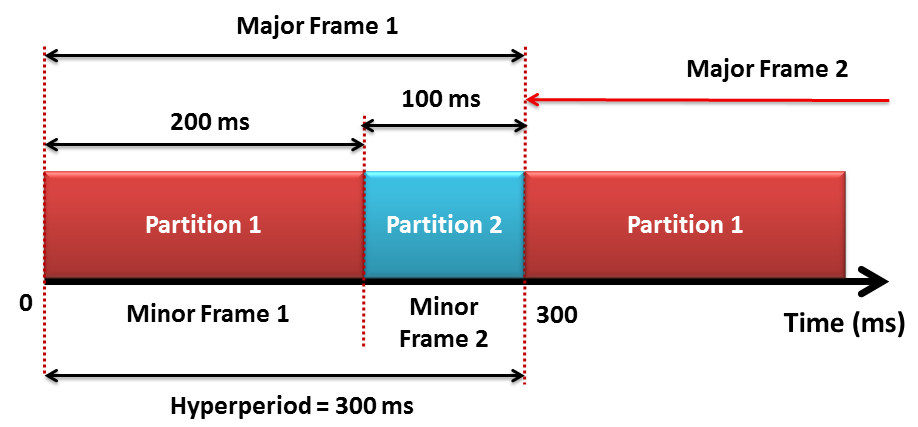
\includegraphics[width=\textwidth]{partition_scheduling}
	\caption{Sample Temporal Partition Schedule with Hyperperiod = 300 ms}
	\label{fig:partition_scheduling}
\end{figure}


Temporal partitions are periodic fixed intervals of the CPU's time. Threads associated with a partition are scheduled only when the partition is active. This enforces a temporal isolation between processes assigned to different partitions. The repeating partition windows are called \emph{minor frames}. The aggregate of repeating minor frames is called a \emph{major frame}. The duration of a major frame is called the \emph{hyperperiod}, which is typically the lowest common multiple of the partition periods. Each minor frame is characterized by a period and a duration. The period specifies how often this partition becomes active and the duration defines how much of the CPU time is available for scheduling the runnable threads associated with that partition. Figure \ref{fig:partition_scheduling} shows a sample temporal partition schedule. By confining applications to partitions i.e. its own memory space and temporal window of possession of computing resources, this scheduling scheme aims to guarantee safety and timeliness in mission-critical systems; safety by isolating processes in different applications and security levels from interacting with each other, and timeliness by providing processes with a guaranteed slice of the CPU time. 
 

%The DREMS component model supports non-functional properties e.g. timeliness, fault tolerance and security as an integral part of the design. Every operation on a component is associated with a deadline. Timed triggers can be associated with operations/callbacks that dictate when and how frequently certain operations are scheduled. Deadline monitoring is invoked when an operation is allowed to execute i.e. enqueued on the component message queue. The component thread that releases the business logic execution thread monitors the deadline. If a hard deadline is reached but the operation is incomplete, then the infrastructure notifies a local fault manager and appropriate actions are taken. 

\section{Motivation to use DREMS}

DREMS supports a wide variety of interaction patterns: synchronous and asynchronous service-oriented request-response style communication, and non-blocking anonymous publish-subscribe style communication. The wide variety of interactions and communication mechanisms are inspired by other common industrial component models such as CIAO \cite{CIAO_Chap:04} and ACM \cite{ACM_SPE:10}, and the execution semantics are precisely defined and implemented. A qualitative evaluation of its capabilities \cite{ISIS_F6_ISORC:13} show that although the model was designed for fractionated spacecraft, DREMS is suitable for a variety of distributed and embedded environments. All of these properties make this component model very generic and a suitable target for the timing analysis work presented in this thesis. 

%Since the component operation scheduling is non-preemptive, it is possible that the operation in the front of the component message queue is blocked for prolonged periods of time by the currently executing operation e.g. the executing operation could be blocked, waiting on some I/O device. In such scenarios, developers can opt into using asynchronous non-blocking I/O operations. 

%Since the component execution semantics allows only one active operation to execute at a time within a component, it is possible that a ready operation is blocked for prolonged periods of time by an operation waiting on some I/O device. In such scenarios, developers can opt into using blocking I/O operations, polling mechanisms and asynchronous nonblocking I/O operations. In a blocking I/O task, the component is unavailable while the operation is running. Other components may execute in the system, but the one waiting on an I/O device is blocked. This blocking could propagate to other components and introduce significant delays. When using polling, some periodic task is scheduled that checks for the completion of I/O interaction. This leads to a potential waste of resources and decreased performance. Lastly, the component model supports asynchronous I/O, where the component triggers an I/O interaction and returns to handle other operations in the queue. The component does not block on the I/O and is notified when the I/O task completes. 